\chapter{22/08/2013 Week}\label{C:us}

\section{Progress}

Got lots more data, scrapers running since Monday (couldn't do earlier due QUAKE!!!). LinkedIn scraper is now functioning, but currently broken because I started adding multi-threading. This shouldn't take long at all to fix. 

\subsection{LinkedIn}
Things I can fetch from publicly-viewable pages: 

\begin{itemize}
 \item number of connections
 \item Number of recommendations
 \item Current Position (creepy?)
 \item Number of skills listed (Often maxed out at 50)
 \item Number of groups/societies that the person has listed
\end{itemize}

\noindent Some of these could be useful/interesting to look at while others might not be (e.g. number of skills, this can just be spammed out.) Could maybe look at relationships between number of skills v recommendations, connections v recommendations.\\

\noindent It's interesting how straightforward pages such as LinkedIn are to scrape vs ones like Twitter or Facebook. Whereas twitter has some dynamic content (e.g. sepearate http request to load detailed tweet data, infinite scroll) which were challenging and time-consuming to make robust, LinkedIn does not. This is another thing I can talk about in report, some form of recommendations about easily-scrapable web pages. It seems obvious now, but it was not obvious when I was starting x many months ago. 

\section{Policies -Data Fetching!!}

Since Monday, scraped lots more profiles... ~600 were collected into this for analysis, but I have done ~800 total. These are more accurate scrapes than previous versions, given a silly bug including tweets that were actually not originally from the author in past results. So I cannot reliably use data from old scrapes too much. That's OK though - performance is much much better now. 

\subsection{Correlation of Impact Factor vs Bucketed Impacts}

\begin{figure}[h!]
\centering
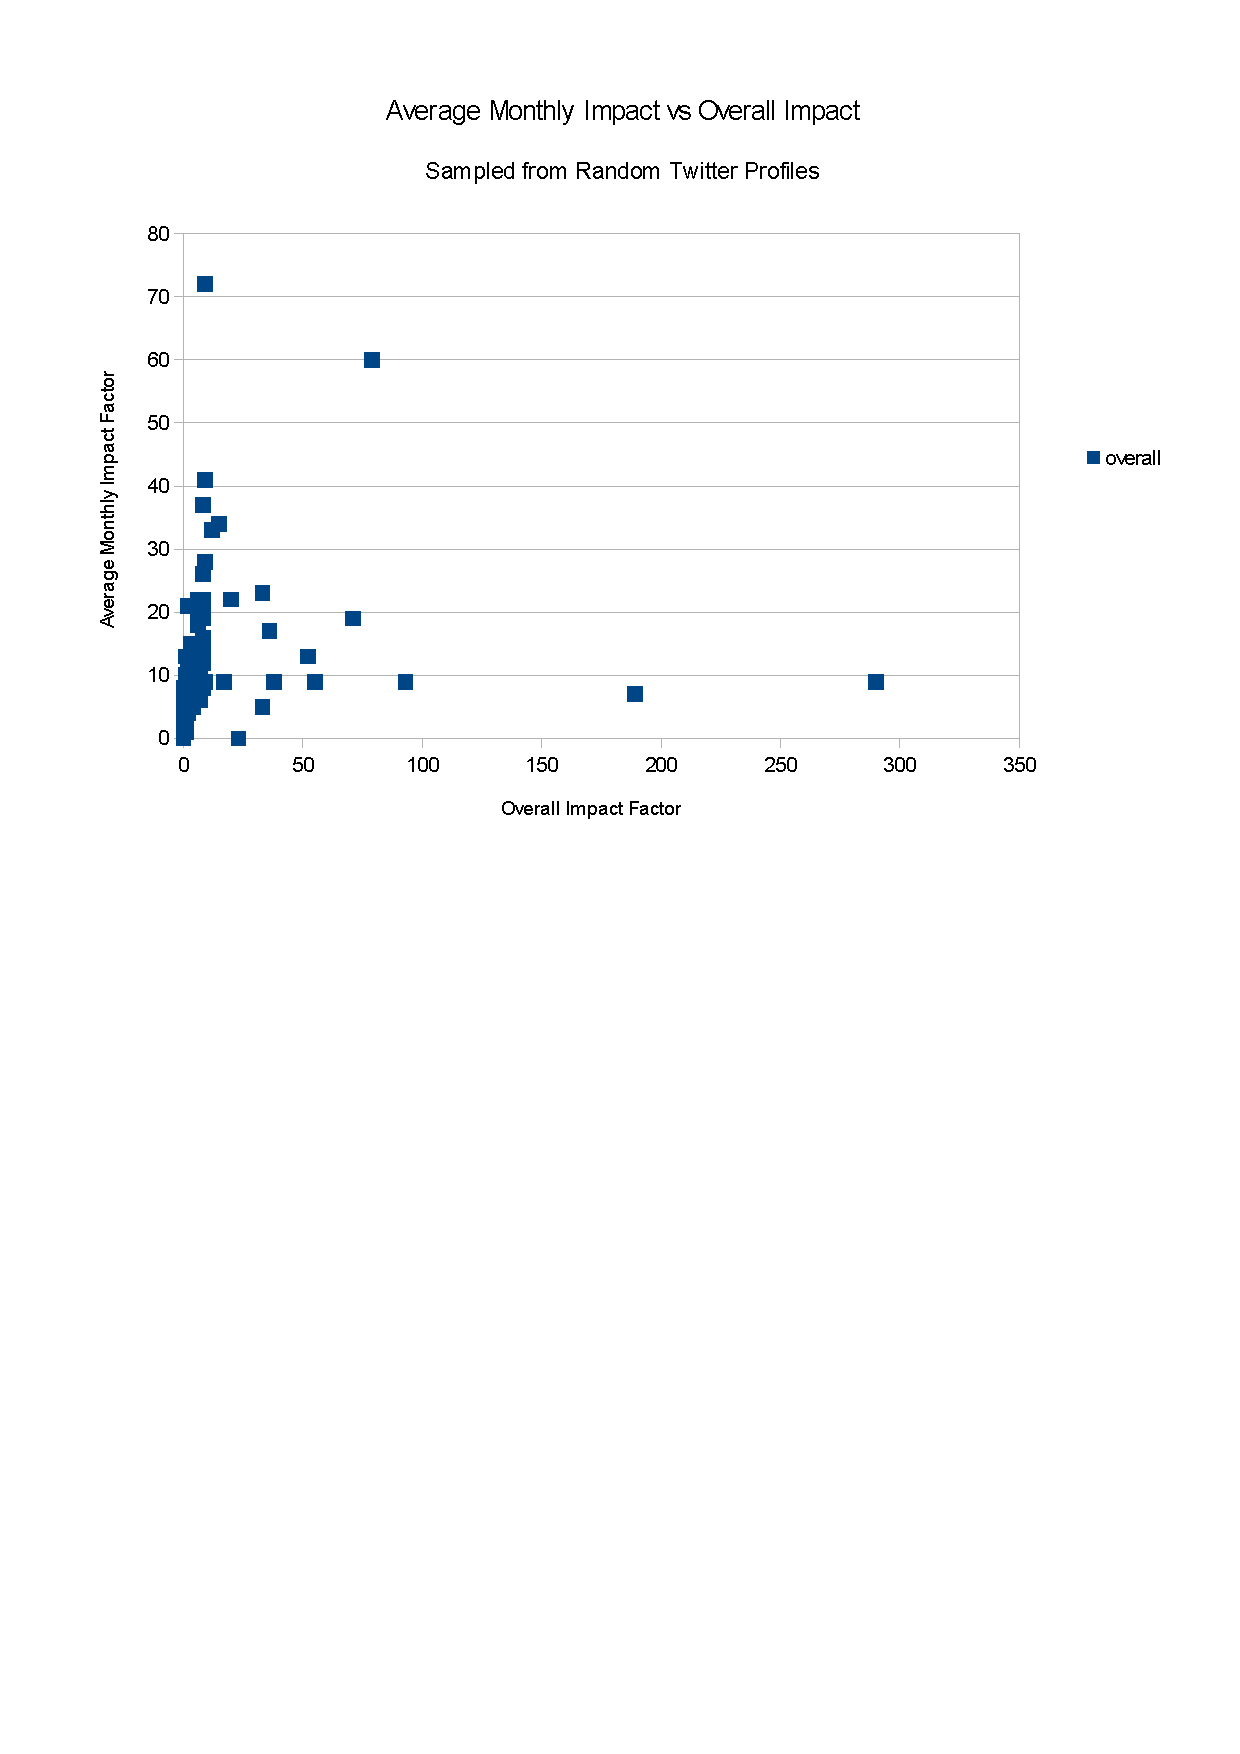
\includegraphics[width=400px]{Images/monthly_impact_vs_overallv2.pdf}
\caption{Monthly Impact against Overall Impact}
\end{figure}

\begin{figure}[h!]
\centering
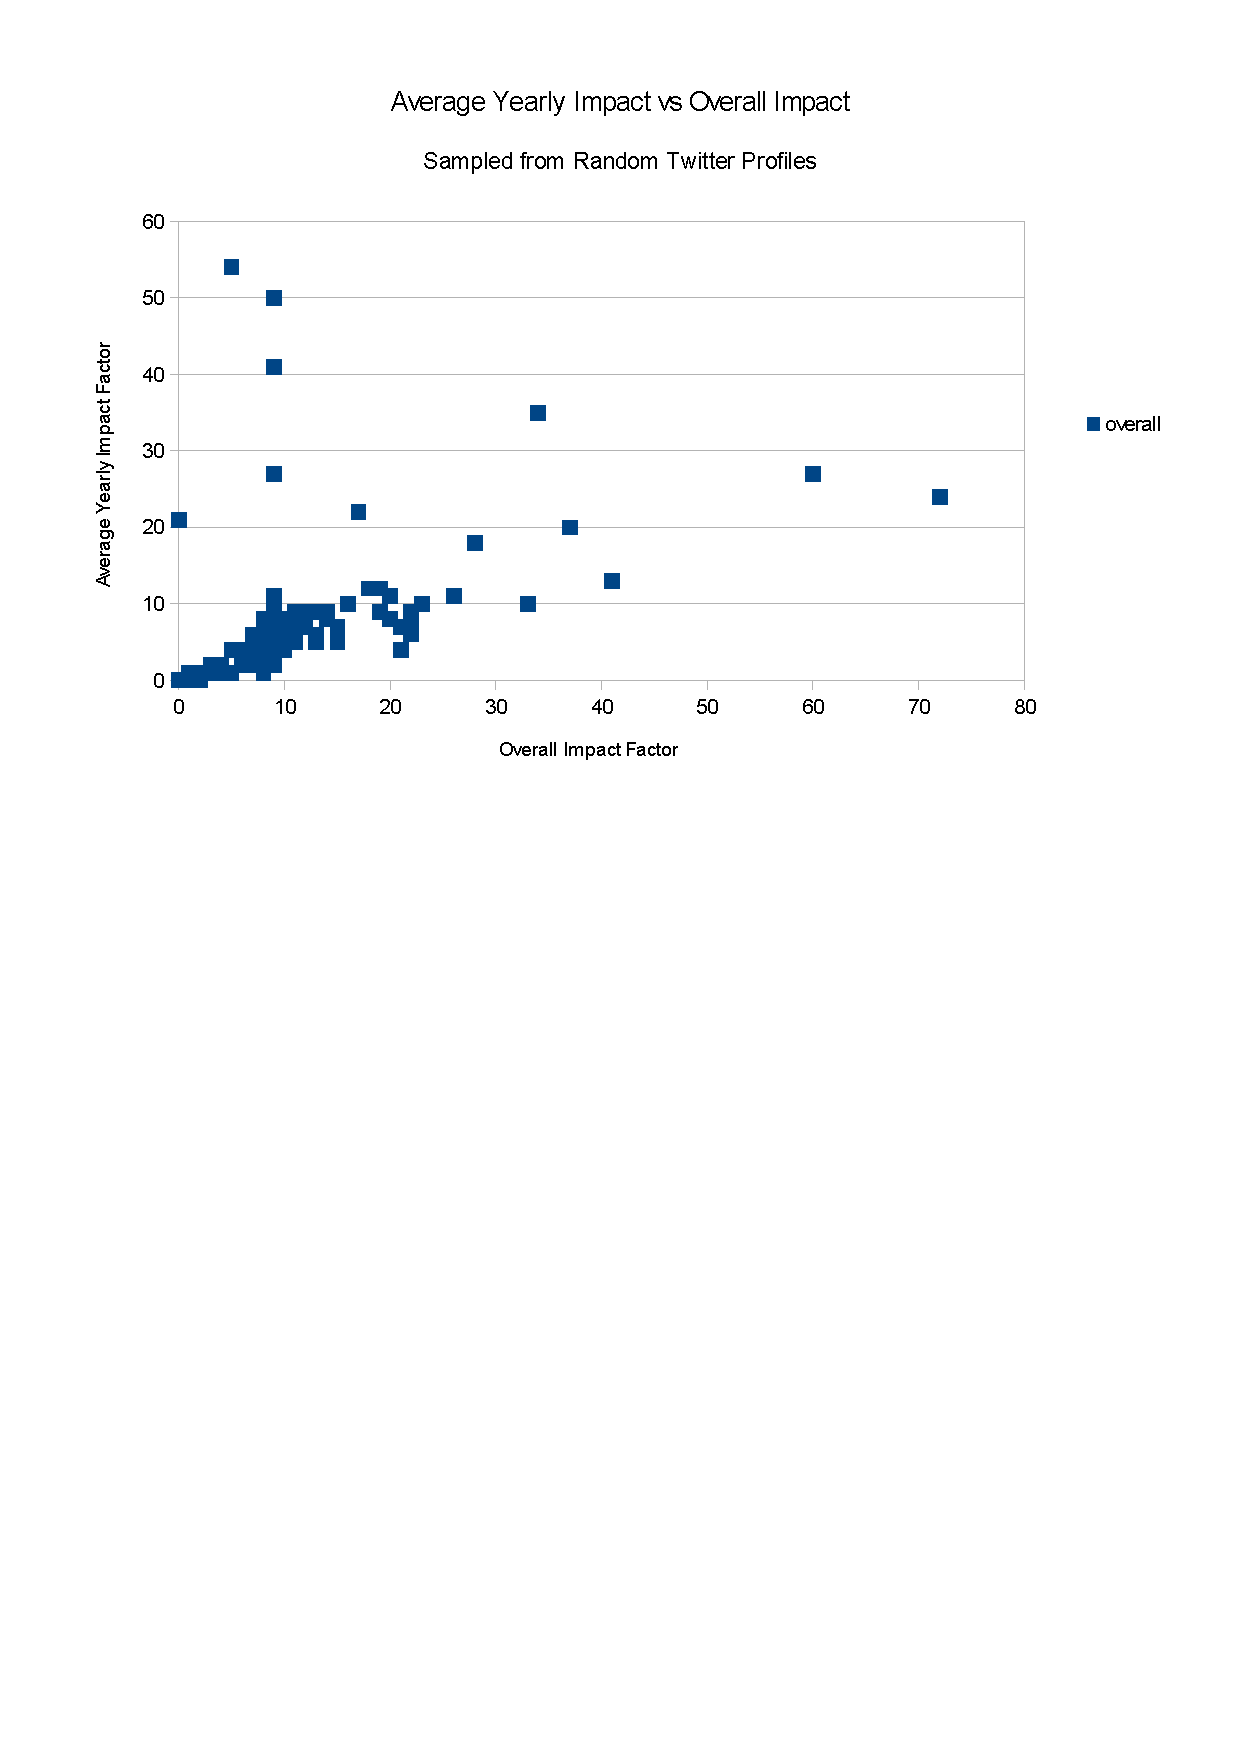
\includegraphics[width=400px]{Images/yearly_impact_vs_overallv2.pdf}
\caption{Yearly Impact against Overall Impact}
\end{figure}

One strategy for inferring reputation information that I looked at was through temporal bucketing of impact factor, into days, months, and years. The figures below show the relationship between people's mean monthly calculated impact factor (i.e. by calculating a person's impact score for each month, and then averaging these values over the total number of months), and the individual's overall impact score. I infer that there is a weak relationship between average monthly impact and overall impact (Pearson's correlation coefficient r= 0.273(3 s.f.)), and a stronger relationship between average yearly impact and overall impact (r=0.689(3 s.f.))\\

\noindent What I believe this data shows is that the impact factor is favourable to individuals who are consistent on Twitter over time. <- Need to back this up

\subsection{Results of Monthly Bucketing}

By applying the impact factor formula to individuals on a monthly basis, we are able to generate an impression of how regularly active a person is. The data also reveals how influential the person has been per month. This assists when comparing individuals who are consistently strongly influential (e.g. Barack Obama, companies such as instagram), with those who are popular for a limited period only. I looked at comparing different bucket sizes for this temporal aggregation. Days, months, and years were used as buckets, with monthly aggregation clearly showing the strongest and more interesting trends. 

\subsubsection{Twitter Scraper Performance}
I evaluate the performance of my twitter scraper with respect to average time taken to fetch and parse a tweet. The major limiting factor for scraping twitter was that each tweet had to be fetched with a seperate http request. Figure <x> shows the average time taken to fetch and parse each tweet, with respect to my incremental build stages. The success of continuous and incremental improvement in performance helps justify my decision to use an incremental approach. Tweets were gathered over several days, and continuously throughout different times of the day on the Victoria network to ensure that a representative range of times were gathered for each stage.\\

\noindent The significant feature of improved performance was through parellization of tweet-fetches. 

\begin{figure}[h!]
\centering
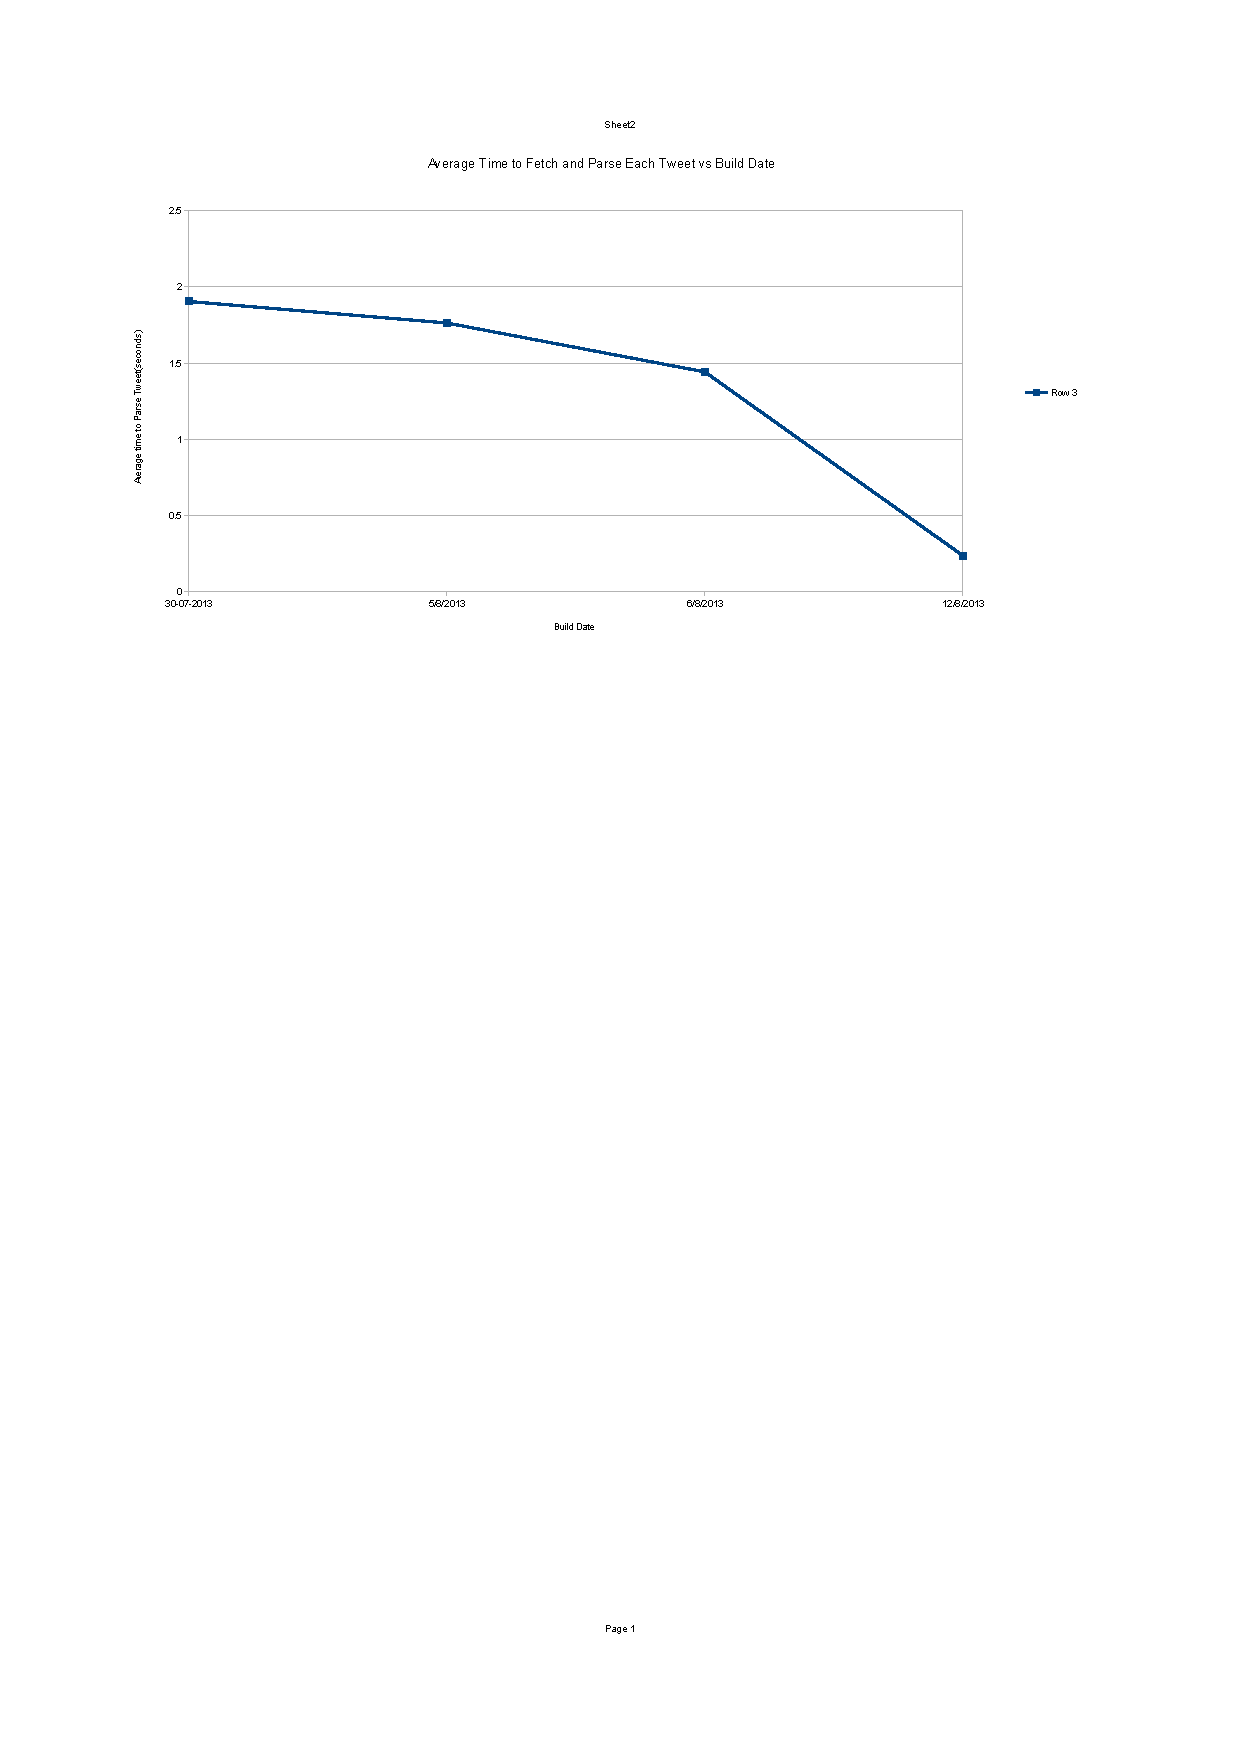
\includegraphics{Images/average_time_to_fetch_parse_tweets_per_build.pdf}
\caption{The Average Time to Fetch and Parse a Tweet, Ordered by Builds}
\end{figure}

Absolute limitations - Every tweet has to be fetched in an individual http request. This produces upper limits as to how fast the scraper can go, and means that the majority of performance speed is reliant on the speed of the network. (data - show how on some days tweets are fetched slightly faster than on other days. Times of day.)


\subsubsection{Ability to Resist Blocking Detection}

The primary measure of my scraper libraries avoiding blocking detection is with regards to their failure or incomplete-scrape rates. Although in early, less stable builds I had parsing errors, my later work only failed when detected by twitter and blocked. As such detection rates in later builds can reliably be calculated by analysing failing or incomplete twitter profiles. 

\begin{figure}[h!]
\centering
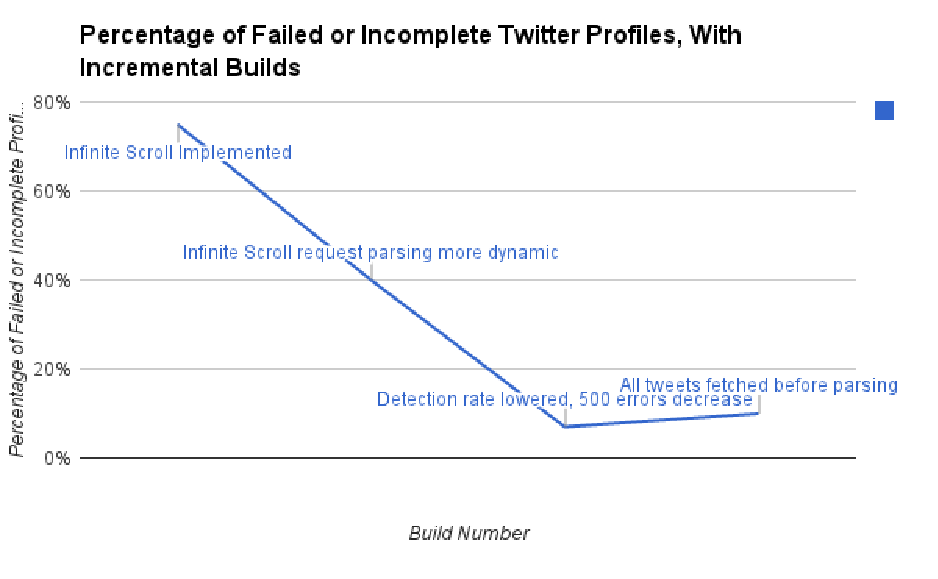
\includegraphics{Images/percentage_failed_incomplete_twitter_profiles.pdf}
\caption{The Percentage of Incomplete or Failed Profile Scrapes, Ordered by Builds}
\end{figure}

\subsubsection{Privacy Protection}

Privacy protection - this is still pretty poor, saved as structured xml, data not anonymised (makes my life easier at present)... Are there things I could be doing here potentially to increase privacy for individuals that I am scraping? Document locking, or store as RDB? Although storage into GRAft would require community effort/a business model and is therefore unlikely, it might add value to my report to demonstrate how this would be feasible through better privacy measures. 
